% \glsresetall
\chapter{Presentation of the results} % Main chapter title
\label{Chapter7}

\lhead{Chapter 7. \emph{Presentation of the results}}

In this chapter it will be explained how and which data was collected using the prototype, and which metrics were defined for comparison.
Afterwards, the landscapes will be compared, using the defined metrics as KPIs. The conclusion based on the results will be given in chapter \ref{Chapter8}.

\section{Basis of the experiment} 

This section will contain information about the environment in which the experiment was executed, how the data was collected and which metrics were defined based on the gathered data.

\subsection{Testing hardware and environment}

It has to be mentioned, that certain aspects of the environment were not maintained by the tester and are, therefore, out of scope for influence or configuration. Nonetheless, they are mentioned here for reproducibility.
The following hardware and environment was used for testing:
\begin{enumerate}[noitemsep]
	\item \textbf{Laptop:} MacBook Pro (15-inch, 2017)
	\begin{itemize}[noitemsep]
		\item \textbf{Processor:} 2.9 GHz Quad-Core Intel Core i7
		\item \textbf{Memory:} 16 GB 2133 MHz LPDDR3 
		\item \textbf{Graphics:} Radeon Pro 560 4 GB and Intel HD Graphics 630 1536 MB
		\item \textbf{macOS Monetary - Version:} 12.2.1 (21D62)
	\end{itemize} 
	
	\item \textbf{Browser, Network and Lighthouse:}
	\begin{itemize}[noitemsep]
		\item \textbf{Browser:} Google Chrome
		\item \textbf{Version:} 99.0.4844.51 (Official Build) (x86\_64)
		\item \textbf{Chrome DevTools version:} Chrome 99
		\item \textbf{Lighthouse version:} 100.0.0.0
		\item \textbf{JavaScript version:} V8 9.9.115.8
		\item \textbf{Network-Bandwidth:} 180-200 Mb/s
	\end{itemize}
	
	\item \textbf{Runtime environment for prototypes:} surge.sh \footnote{surge.sh is a platform for static web publishing
		for frontend developers via the command line.}
	
	\item \textbf{CDN:} Unpkg.com \footnote{This part of the environment was explained in chapter \ref{Chapter6}}
\end{enumerate}

In addition to the specified hardware specs, version 1.18.1 of the \texttt{@luigi-project} was used. This dependency enables the Luigi framework and is, therefore, used in every implemented version of the prototype.

\subsection{Testing process}

Since multiple Nodes were implemented, a unified process was required to collect comparable data. The BPMN diagram \ref{fig:data_collection_process_har} contains the process steps in detail.

\begin{figure}[!h]
	\centering
	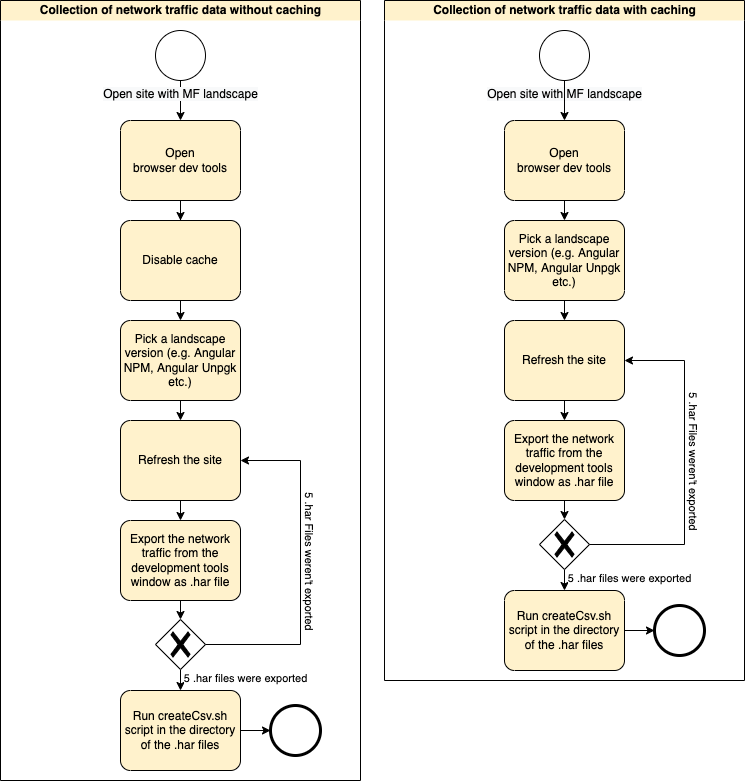
\includegraphics[width=0.7\textwidth]{Figures/Data_Collection_Process_har.drawio.png}
	\caption{Data collection process for .har files}
	\label{fig:data_collection_process_har}
\end{figure}

As it can be seen in \ref{fig:data_collection_process_har}, there were actually two processes executed to collect data. 
The first one had caching disabled, the second one enabled. 
The intention behind the first process was to collect data for an average initial loading time for the picked site, therefore, the resources must not be cached. 
The second process was used to gather information about caching behavior in general. 
Since each Node basically contains the same views, the browser should be able to pull already loaded resources from the cache, instead via the network. 
To showcase this behavior and prove the performance gain through caching, this data was gathered too.
Each process was executed 5 times, therefore 10 HTTP Archive (\texttt{.har}) files were generated per Node. 
These \texttt{.har} files were then transformed into \texttt{.csv} files using a self-developed script, which can be found in the archive.

Additionally to the \texttt{.har} files, a website performance report was collected, using the Lighthouse tool embedded in the Google Chrome browser. Such a report provides information about the usage of the imported bytes by a web application, distinguished by resource URL.

In summary, for testing:

\begin{itemize}[noitemsep]
	\item 12 Nodes were developed.
	\item Each Node was loaded 10 times, 5 times with cache enabled and 5 times with cache disabled.
	\item Each loading of a Node is represented by a HTTP Archive file.
	\item The testing procedures were executed 120 times overall.
	\item 120 \texttt{.har} files were generated.
	\item These, were aggregated and transformed into 12 \texttt{.csv} files.
	\item These, were copied into one Excel file, where the data was analyzed.
	\item In addition, 12 Lighthouse reports where collected (one per Node) and added to the Excel.
\end{itemize}

The reason why this testing procedure was chosen, was due to the low variety in the parameters when a Node is loaded. 
First, it was tested if the parameters would vary when a Node is loaded up to 1000 times, which was found to be not the case. 
Due the constant resource sizes and stable network, not many fluctuations could be observed. 
Only when changes on technological level were made (e.g. usage of cache, network outage), fluctuations started to appear. 
But, other than that, it was observed that the results were stable. Therefore, it was decided that loading a Node 10 times would suffice for the experiment.

After the collection process, another self-developed script was used to aggregate all the gathered data into one single file. This file was later used to define and calculate the metrics, which are described next.

\subsection{Defined metrics}
\label{metric_definition}
The central file, containing all data, was split into separate sheets in which the metrics for each micro frontend were calculated. The parameters for calculation were:

\begin{description}
	\item[connection:] This is an ID for each opened TCP connection provided by the browser. It can be an indicator for the parallelity of the requests. Since the release of HTTP/2, several requests can be handled by a server via the same TCP connection, reducing the number for TCP handshakes. The application requesting the sources can not implement this HTTP/2 feature. It has to be enabled on server-side and by the browser, which is already the case for most modern browsers \cite{http2}. As of today, surge.sh, the web server platform onto which the prototypes are deployed, does not support HTTP/2.
	
	\item[loadedFromCache:] This is a string value with three possible characteristics, \textit{not loaded from cache, disk} or \textit{memory}, whereas \textit{disk} and \textit{memory} are semantically the same for the context of this thesis. This value explains from where the resource was loaded. Either via the network from a server or from the local cache. It indicates the caching behavior of bundled resources, in comparison with resources loaded from a unified URL (e.g. a CDN). 
	
	\item[startedDateTime:] This is a timestamp given to each request, marking its starting time in a DateTime format. This value can serve as an indicator for parallelity, since multiple TCP connections can be opened at the same time. 
	
	\item[requestUrl:] This is a string value, containing the request URL used by the browser to load the resource. This value mainly categorizes the calculation results, since neither \textit{connection} nor \textit{pageRef} are valid options to distinguish the loaded resources of a website. 
	
	\item[responseContentSize:] This number value is the byte size of the loaded resource.
	
	\item[timeInMs:] This value represents the RTT of the request in milliseconds. 
\end{description}

Further were parameters, available in the \texttt{.har} files, but those could not be used for the calculation, since those were either to application-specific or had no significance for the goal of this thesis.
Based on the given metrics from the \texttt{.har} files, the following KPIs were calculated.

\begin{description} 
	\item[Avg. content size:] Numerical value calculated by averaging the \textbf{responseContentSize} values of all the websites resources.
	
	\item[Avg. time in MS loaded values:] Numerical value, calculated by averaging the \newline \textbf{timeInMs} values of all the websites resources.
	
	\item[Occurrences connection duplicates:] Numerical value to represent parallelity, by counting the number of duplicate/multiple occurring \textbf{connection} values.
	
	\item[Connection IDs:] List of all \textbf{connection} characteristics for the website.
	
	\item[Connection IDs occurrence:] Number of times the \textbf{connection} occurred during the loading of the website.
	
	\item[Parallel start time:] Numerical value, calculated by counting reoccurring \textbf{startedDateTime} values.
	
	\item[Avg. response content size per loading type:] Numerical value, calculated by averaging the \textbf{responseContentSize}, differentiated by the characteristics of the \textbf{loadedFromCache} property.
	
	\item[URLs loaded:] List of all unique \textbf{requestUrl} values.
	
	\item[Avg. response time per URL loaded in MS:] Numerical value, representing the average loading time of each loaded resource URL of the website.
	
	\item[Avg. response size per URL loaded:] Numerical value, representing the average loading byte size of each resource URL.
	
	\item[Avg. response size per URL loaded via network:] Numerical value, calculated by averaging the \textbf{responseContentSize} differentiated by the \textbf{requestUrl} for all resources with the \textbf{loadedFromCache} value of \textit{not loaded from cache}. For the test scenarios with cache disabled, this value equals the \textbf{Avg. Response Size per URL loaded} KPI.
	
	\item[Avg. response size per URL loaded from disk:] Numerical value, calculated by averaging the \textbf{responseContentSize} differentiated by the \textbf{requestUrl}, for all resources with the \textbf{loadedFromCache} value of \textit{disk}.
	
	\item[Avg. response size per URL loaded from memory:] Numerical value, calculated by averaging the \textbf{responseContentSize} differentiated by the \textbf{requestUrl}, for all resources with the \textbf{loadedFromCache} value of \textit{memory}.
\end{description}

The main indicators for whether a technology successfully reduces redundant libraries in a micro frontend landscapes were the \textbf{Avg. time in MS loaded values} and \textbf{Avg. content size}.

\textbf{Avg. content size} was chosen as a main indicator, due to its significance. The reduction in loaded libraries, should be represented in the overall loaded byte size. Therefore, this metric is object for optimization.

\textbf{Avg. time in MS loaded values} was chosen as the second main indicator, since it is asserted that the loading time correlates with the bytes loaded by a micro frontend. It can be argued, that this value also correlates strongly with the bandwidth of the testing environment. However, it still was chosen, since it is a metric for optimization. The goal of reducing redundancies in a micro frontend landscape is considered to be achieved, when the number of loaded bytes and the loading time of a website are decreased.
If a technology avoids redundant libraries in a micro frontend landscape, but increases the loading time of that landscape, the result is insufficient for the purpose of this transcript.

Therefore, the goal was to optimize these two KPIs. If, by using a technology, these two values decreased, it was considered to be a first success. 
But, for the general evaluation, further aspects were put into consideration. 
KPIs for those aspects, such as e.g. the complexity of the implemented technology, were hard to measure.  
A metric like this must not be ignored for the context of this transcript, since the benefit of a technology highly depends on it.
Thus, the subjective estimation and impression of the used technologies by the author is part of the conclusion in chapter \ref{Chapter8}.

Statistical values, like the median of loading times or loaded bytes, were calculated, but not included in the conclusion, since the meaningfulness of those values was not applicable for the goal. The package size does affect loading time of a resources, that is a matter of fact. But since the packages are application-specific, no general statement can be drawn from the median of this parameters. The goal was to showcase that through the use of one of the three technologies, the loading times and loaded bytes are reduced in general, not to show what package was not loaded or loaded faster.

In the following sections, the results of the introduced metrics for each landscape are showcased. 
The tables shown, are separated whether, the data was collected with caching enabled or disabled. 
In addition, to the shown metrics, the graphs and Excel tables for the landscapes are referred to in the archive.
A table of contents of the archive is available in appendix \ref{appendix1}.

\section{CDN/NPM KPI results}

This section will introduce the KPI results of the CDN/NPM prototype. It is split into 2 subsections for a better comparison of the two technologies.

\subsection{Implementation with NPM}

Table \ref{tab:cdn_result_table} contains the results for the implemented Nodes with a regular bundler and a package manager, namely NPM. 
Certain metrics are not added to the table for readability (cf. \ref{metric_definition}), but those, as well as a graphical representation, can be found in archive. 

\scriptsize
\setlength{\mycolwidth}{\dimexpr \textwidth/5 - 2\tabcolsep}

\begin{longtable}[c]{*{3}{p{\mycolwidth}}}
	
	\caption{Table of numerical KPI results for the NPM Nodes with caching disabled}
	\label{tab:cdn_result_table} \\
	
	\toprule
	\multicolumn{1}{l}{\makecell[c]{\textbf{Metric}}}   
	& \multicolumn{1}{l}{\makecell[c]{\textbf{Angular NPM}}}                              
	& \multicolumn{1}{l}{\makecell[c]{\textbf{Vue NPM}}} \\ 
	\midrule
	\endfirsthead
	
	\multicolumn{3}{l}{\footnotesize\itshape\tablename~\thetable:
		continued from previous page} \\
	\toprule   
	\multicolumn{1}{l}{\makecell[c]{\textbf{Metric}}}   
	& \multicolumn{1}{l}{\makecell[c]{\textbf{Angular NPM}}}                              
	& \multicolumn{1}{l}{\makecell[c]{\textbf{Vue NPM}}} \\*
	\midrule
	\endhead
	%		
	\multicolumn{1}{l|}{URLs loaded count}                                         															
	& \multicolumn{1}{l|}{\makecell[c]{14}} 	
	& \multicolumn{1}{l}{\makecell[c]{13}}   \\ \midrule
	
	\multicolumn{1}{l|}{\makecell[l]{Avg. response content size\\per loading type}}   
	& \multicolumn{1}{l|}{\makecell[c]{\textit{not loaded from cache:} 129529.13 \\ \textit{memory:} 0, \\ \textit{disk:} 0}} 											
	& \multicolumn{1}{l}{\makecell[c]{\textit{not loaded from cache:} 156131.63 \\ \textit{memory:} 0, \\ \textit{disk:} 0}}   \\ \midrule
	
	\multicolumn{1}{l|}{Parallel start time}                                 													
	& \multicolumn{1}{l|}{\makecell[c]{33}} 				
	& \multicolumn{1}{l}{\makecell[c]{45}}   \\ \midrule
	
	\multicolumn{1}{l|}{Connection IDs occurence}                            											
	& \multicolumn{1}{l|}{\makecell[c]{\textit{none established:} 10,\\ \textit{207393:} 10}} 												   
	& \multicolumn{1}{l}{\makecell[c]{\textit{241394:} 10}}   \\ \midrule
	
	\multicolumn{1}{l|}{Connection IDs count}                                      																
	& \multicolumn{1}{l|}{\makecell[c]{62}} 															     
	& \multicolumn{1}{l}{\makecell[c]{71}}   \\ \midrule
		
	\multicolumn{1}{l|}{\makecell[l]{Connection duplicates}}                        
	& \multicolumn{1}{l|}{\makecell[c]{20}} 						   
	& \multicolumn{1}{l}{\makecell[c]{10}}   \\ \midrule
	
	\multicolumn{1}{l|}{\makecell[l]{Loaded values \& occurrences}}                        
	& \multicolumn{1}{c|}{\makecell[c]{\textit{not loaded from cache:} 80,\\ \textit{memory:} 0, \\ \textit{disk:} 0}} 						   
	& \multicolumn{1}{l}{\makecell[c]{\textit{not loaded from cache:} 80, \\ \textit{memory:} 0, \\ \textit{disk:} 0}}   \\ \midrule
	
	\multicolumn{1}{l|}{\makecell[l]{Avg. time in MS}}                        
	& \multicolumn{1}{l|}{\makecell[c]{162.22}} 						   
	& \multicolumn{1}{l}{\makecell[c]{5323.54}}   \\ \midrule
	
	\multicolumn{1}{l|}{\makecell[l]{Avg. content size}}                                         
	& \multicolumn{1}{l|}{\makecell[c]{129529.13}}  				  
	&   \multicolumn{1}{l}{\makecell[c]{156131.63}} \\ \bottomrule
\end{longtable}

\normalsize
The results shown in table \ref{tab:cdn_result_table} were collected without caching enabled. 
This explains for instance, why no resources were loaded from cache and therefore, why the values for the \textit{memory} or \textit{disk} characteristics are missing.
The main takeaway from these results is an average initial loading time for the Nodes, which differs depending on the framework. 
It can also be seen that even though fewer resources are loaded via URLs by the Vue.js Nodes, they have a longer loading time compared to the Angular ones.

\scriptsize
\setlength{\mycolwidth}{\dimexpr \textwidth/5 - 2\tabcolsep}

\begin{longtable}[c]{*{3}{p{\mycolwidth}}}
	
	\caption{Table of numerical KPI results for the NPM Nodes with caching enabled}
	\label{tab:cdn_result_table_caching} \\
	
	\toprule
	\multicolumn{1}{l}{\makecell[c]{\textbf{Metric}}}   
	& \multicolumn{1}{l}{\makecell[c]{\textbf{Angular NPM}}}                              
	& \multicolumn{1}{l}{\makecell[c]{\textbf{Vue NPM}}} \\ 
	\midrule
	\endfirsthead
	
	\multicolumn{3}{l}{\footnotesize\itshape\tablename~\thetable:
		continued from previous page} \\
	\toprule   
	\multicolumn{1}{l}{\makecell[c]{\textbf{Metric}}}   
	& \multicolumn{1}{l}{\makecell[c]{\textbf{Angular NPM}}}                              
	& \multicolumn{1}{l}{\makecell[c]{\textbf{Vue NPM}}} \\*
	\midrule
	\endhead
	%		
	\multicolumn{1}{l|}{URLs loaded count}                                         															
	& \multicolumn{1}{l|}{\makecell[c]{14}} 	
	& \multicolumn{1}{l}{\makecell[c]{13}}   \\ \midrule
	
	\multicolumn{1}{l|}{\makecell[l]{Avg. response content size\\per loading type}}   
	& \multicolumn{1}{l|}{\makecell[c]{\textit{not loaded from cache:} 166856, \\ \textit{memory:} 17548.5, \\ \textit{disk:} 17548.5}} 											
	& \multicolumn{1}{l}{\makecell[c]{\textit{not loaded from cache:} 145646.67,\\ \textit{memory:} 0, \\ \textit{disk:} 187586.5}}   \\ \midrule
	
	\multicolumn{1}{l|}{Parallel start time}                                 													
	& \multicolumn{1}{l|}{\makecell[c]{32}} 				
	& \multicolumn{1}{l}{\makecell[c]{39}}   \\ \midrule
	
	\multicolumn{1}{l|}{Connection IDs occurence}                            											
	& \multicolumn{1}{l|}{\makecell[c]{\textit{none established:}20}} 												   
	& \multicolumn{1}{l}{\makecell[c]{\textit{none established:}20}}   \\ \midrule
	
	\multicolumn{1}{l|}{Connection IDs count}                                      																
	& \multicolumn{1}{l|}{\makecell[c]{61}} 															     
	& \multicolumn{1}{l}{\makecell[c]{61}}   \\ \midrule
	
	\multicolumn{1}{l|}{\makecell[l]{Connection duplicates}}                        
	& \multicolumn{1}{l|}{\makecell[c]{20}} 						   
	& \multicolumn{1}{l}{\makecell[c]{20}}   \\ \midrule
	
	\multicolumn{1}{l|}{\makecell[l]{Loaded values \& occurrences}}                        
	& \multicolumn{1}{c|}{\makecell[c]{\textit{not loaded from cache:} 60, \\ \textit{memory:} 6, \\ \textit{disk:} 14}} 						   
	& \multicolumn{1}{l}{\makecell[c]{\textit{not loaded from cache:} 60, \\ \textit{memory:} 0, \\ \textit{disk:} 20}}   \\ \midrule
	
	\multicolumn{1}{l|}{\makecell[l]{Avg. time in MS}}                        
	& \multicolumn{1}{l|}{\makecell[c]{150.90}} 						   
	& \multicolumn{1}{l}{\makecell[c]{1890.6}}   \\ \midrule
	
	\multicolumn{1}{l|}{\makecell[l]{Avg. content size}}                                         
	& \multicolumn{1}{l|}{\makecell[c]{129529.13}}  				  
	&   \multicolumn{1}{l}{\makecell[c]{156131.63}} \\ \bottomrule
	
\end{longtable}

\normalsize
The results of table \ref{tab:cdn_result_table_caching} show the effect caching has on the performance of a site. 
The average loading time of the site decreases, as do the opened TCP connections.

Both environments were implemented using a regular bundler. Therefore, it cannot be ensured that redundant libraries were not loaded.

\subsection{Implementation with Unpkg.com}

Table \ref{tab:cdn_result_table_unpkg} contains the results for the implemented Nodes with a use of a public CDN, namely Unpkg.com. 
Certain metrics are not added to the table for readability, but those, as well as a graphical representation, can be found in archive. 

\scriptsize
\setlength{\mycolwidth}{\dimexpr \textwidth/5 - 2\tabcolsep}

\begin{longtable}[c]{*{3}{p{\mycolwidth}}}
	
	\caption{Table of numerical KPI results for the Nodes using the Unpkg.com CDN with caching disabled}
	\label{tab:cdn_result_table_unpkg} \\
	
	\toprule
	\multicolumn{1}{l}{\makecell[c]{\textbf{Metric}}}   
	& \multicolumn{1}{l}{\makecell[c]{\textbf{Angular Unpkg}}}                              
	& \multicolumn{1}{l}{\makecell[c]{\textbf{Vue Unpkg}}} \\ 
	\midrule
	\endfirsthead
	
	\multicolumn{3}{l}{\footnotesize\itshape\tablename~\thetable:
		continued from previous page} \\
	\toprule                        
	\multicolumn{1}{l}{\makecell[c]{\textbf{Metric}}}   
	& \multicolumn{1}{l}{\makecell[c]{\textbf{Angular Unpkg}}}                              
	& \multicolumn{1}{l}{\makecell[c]{\textbf{Vue Unpkg}}} \\*
	\midrule
	\endhead
	%		
	\multicolumn{1}{l|}{URLs loaded count}                                         															
	& \multicolumn{1}{l|}{\makecell[c]{171}} 	
	& \multicolumn{1}{l}{\makecell[c]{165}}   \\ \midrule
	
	\multicolumn{1}{l|}{\makecell[l]{Avg. response content size\\per loading type}}   
	& \multicolumn{1}{l|}{\makecell[c]{\textit{not loaded from cache:} 9768.62, \\ \textit{memory:} 0, \\ \textit{disk:} 0}} 											
	& \multicolumn{1}{l}{\makecell[c]{\textit{not loaded from cache:} 8205.19, \\ \textit{memory:} 0, \\ \textit{disk:} 0}}   \\ \midrule
	
	\multicolumn{1}{l|}{Parallel start time}                                 													
	& \multicolumn{1}{l|}{\makecell[c]{871}} 				
	& \multicolumn{1}{l}{\makecell[c]{989}}   \\ \midrule
	
	\multicolumn{1}{l|}{Connection IDs occurence}                            											
	& \multicolumn{1}{l|}{\makecell[c]{\textit{223736:} 20,\\ \textit{223722:} 1574,\\ \textit{none established:}10}} 												   
	& \multicolumn{1}{l}{\makecell[c]{\textit{241394:}  20,\\ \textit{249654:} 1560}}   \\ \midrule
	
	\multicolumn{1}{l|}{Connection IDs count}                                      																
	& \multicolumn{1}{l|}{\makecell[c]{53}} 															     
	& \multicolumn{1}{l}{\makecell[c]{42}}   \\ \midrule
	
	\multicolumn{1}{l|}{\makecell[l]{Connection duplicates}}                        
	& \multicolumn{1}{l|}{\makecell[c]{1604}} 						   
	& \multicolumn{1}{l}{\makecell[c]{1580}}   \\ \midrule
	
	\multicolumn{1}{l|}{\makecell[l]{Loaded values \&\\ occurrences}}                        
	& \multicolumn{1}{c|}{\makecell[c]{\textit{not loaded from cache:} 1654, \\ \textit{memory:} 0, \\ \textit{disk:} 0}} 						   
	& \multicolumn{1}{l}{\makecell[c]{\textit{not loaded from cache:} 1620, \\ \textit{memory:} 0, \\ \textit{disk:} 0}}   \\ \midrule
	
	\multicolumn{1}{l|}{\makecell[l]{Avg. time in MS}}                        
	& \multicolumn{1}{l|}{\makecell[c]{97.23}} 						   
	& \multicolumn{1}{l}{\makecell[c]{194.01}}   \\ \midrule
	
	\multicolumn{1}{l|}{\makecell[l]{Avg. content size}}                                         
	& \multicolumn{1}{l|}{\makecell[c]{9768.62}}  				  
	&   \multicolumn{1}{l}{\makecell[c]{8205.19}} \\ \bottomrule
	
\end{longtable}

\normalsize
The data shown in table \ref{tab:cdn_result_table_unpkg} has again been collected without caching enabled.
An approximate estimation for the initial loading times can be drawn from this. 
It becomes apparent that the Vue.js environment takes longer to load for less content. 
A similar behavior was observed in the NPM implementations.
Nonetheless, it is an improvement in performance compared to the NPM counterparts for both Nodes. 
The trade-off of this technology is that single component resources, like a button or a table, had to be imported via script tags one by one, thus the increase in loaded URLs.
This also explains the reduction in \textbf{Avg. content size}. The CDN Nodes only request the necessary resources, such as buttons, tables or lists, and avoid loading the whole component libraries.

\scriptsize
\setlength{\mycolwidth}{\dimexpr \textwidth/5 - 2\tabcolsep}

\begin{longtable}[c]{*{3}{p{\mycolwidth}}}
 	
 	\caption{Table of numerical KPI results for the Nodes using the Unpkg.com CDN with caching enabled}
 	\label{tab:cdn_result_table_unpkg_cache} \\
 	
 	\toprule
	\multicolumn{1}{l}{\makecell[c]{\textbf{Metric}}}   
	& \multicolumn{1}{l}{\makecell[c]{\textbf{Angular Unpkg}}}                              
	& \multicolumn{1}{l}{\makecell[c]{\textbf{Vue Unpkg}}} \\ 
 	\midrule
 	\endfirsthead
 	
 	\multicolumn{3}{l}{\footnotesize\itshape\tablename~\thetable:
 		continued from previous page} \\
 	\toprule   
	\multicolumn{1}{l}{\makecell[c]{\textbf{Metric}}}   
	& \multicolumn{1}{l}{\makecell[c]{\textbf{Angular Unpkg}}}                              
	& \multicolumn{1}{l}{\makecell[c]{\textbf{Vue Unpkg}}} \\*
 	\midrule
 	\endhead
 	%		
 	\multicolumn{1}{l|}{URLs loaded count}                                         															
 	& \multicolumn{1}{l|}{\makecell[c]{171}} 	
 	& \multicolumn{1}{l}{\makecell[c]{165}}   \\ \midrule
 	
 	\multicolumn{1}{l|}{\makecell[l]{Avg. response content size\\per loading type}}   
 	& \multicolumn{1}{l|}{\makecell[c]{\textit{not loaded from cache:} 63972.08, \\ \textit{memory:} 208838, \\ \textit{disk:} 7166.1}} 											
 	& \multicolumn{1}{l}{\makecell[c]{\textit{not loaded from cache:} 28143.2, \\ \textit{memory:} 0, \\ \textit{disk:} 7570.22}}   \\ \midrule
 	
 	\multicolumn{1}{l|}{Parallel start time}                                 													
 	& \multicolumn{1}{l|}{\makecell[c]{1111}} 				
 	& \multicolumn{1}{l}{\makecell[c]{1069}}   \\ \midrule
 	
 	\multicolumn{1}{l|}{Connection IDs occurence}                            											
 	& \multicolumn{1}{l|}{\makecell[c]{\textit{none established:} 1590,\\ \textit{223722:} 15}} 												   
 	& \multicolumn{1}{l}{\makecell[c]{\textit{none established:} 1570,\\ \textit{249654:} 10}}   \\ \midrule
 	
 	\multicolumn{1}{l|}{Connection IDs count}                                      																
 	& \multicolumn{1}{l|}{\makecell[c]{52}} 															     
 	& \multicolumn{1}{l}{\makecell[c]{42}}   \\ \midrule
 	
 	\multicolumn{1}{l|}{\makecell[l]{Connection duplicates}}                        
 	& \multicolumn{1}{l|}{\makecell[c]{1605}} 						   
 	& \multicolumn{1}{l}{\makecell[c]{1580}}   \\ \midrule
 	
 	\multicolumn{1}{l|}{\makecell[l]{Loaded values \& occurrences}}                        
 	& \multicolumn{1}{c|}{\makecell[c]{\textit{not loaded from cache:} 65, \\ \textit{memory:} 3, \\ \textit{disk:} 1587}} 						   
 	& \multicolumn{1}{l}{\makecell[c]{\textit{not loaded from cache:} 50, \\ \textit{memory:} 0, \\ \textit{disk:} 1570}}   \\ \midrule
 	
 	\multicolumn{1}{l|}{\makecell[l]{Avg. time in MS}}                        
 	& \multicolumn{1}{l|}{\makecell[c]{58.73}} 						   
 	& \multicolumn{1}{l}{\makecell[c]{87.1}}   \\ \midrule
 	
 	\multicolumn{1}{l|}{\makecell[l]{Avg. content size}}                                         
 	& \multicolumn{1}{l|}{\makecell[c]{9762.72}}  				  
 	&   \multicolumn{1}{l}{\makecell[c]{8205.19}} \\ \bottomrule
 	
\end{longtable}

\normalsize
A similar development can be observed in table \ref{tab:cdn_result_table_unpkg_cache}. Firstly, with caching enabled, the number of loaded resources from cache increases significantly. Secondly, the average loading times decrease, and lastly, the Angular environments show shorter average loading times, despite more resources being requested via URL by them.

\section{Web Components and WMF landscapes}

As described in chapter \ref{Chapter6}, these environments exist in different versions. They were designed that way to showcase how the used technologies handle multi-version landscapes and how they affect the performance.
Table \ref{tab:wmf_compound} shows the KPIs of those environments.
 
\scriptsize
\setlength{\mycolwidth}{\dimexpr \textwidth/5 - 2\tabcolsep}

\begin{longtable}[c]{*{3}{p{\mycolwidth}}}
	
	\caption{Table of numerical KPI results, for the Nodes implemented with Web Components and WMF as compounds, with caching disabled}
	\label{tab:wmf_compound} \\
	
	\toprule
	\multicolumn{1}{l}{\makecell[c]{\textbf{Metric}}}   
	& \multicolumn{1}{l}{\makecell[c]{\textbf{Web Components}}}                              
	& \multicolumn{1}{l}{\makecell[c]{\textbf{WMF}}} \\ 
	\midrule
	\endfirsthead
	
	\multicolumn{3}{l}{\footnotesize\itshape\tablename~\thetable: continued from previous page} \\
	\toprule                        
	\multicolumn{1}{l}{\makecell[c]{\textbf{Metric}}}   
	& \multicolumn{1}{l}{\makecell[c]{\textbf{Web Components}}}                              
	& \multicolumn{1}{l}{\makecell[c]{\textbf{WMF}}} \\*
	\midrule
	\endhead
	%		
	\multicolumn{1}{l|}{URLs loaded count}                                         															
	& \multicolumn{1}{l|}{\makecell[c]{27}} 	       
	& \multicolumn{1}{l}{\makecell[c]{118}}   \\ \midrule
	
	\multicolumn{1}{l|}{\makecell[l]{Avg. response content size\\per loading type}}   
	& \multicolumn{1}{l|}{\makecell[c]{\textit{not loaded from cache:} 213266.74, \\ \textit{memory:} 0,\\ \textit{disk:} 0}} 			         
	& \multicolumn{1}{l}{\makecell[c]{\textit{not loaded from cache:} 507168.76, \\ \textit{memory:} 0, \\ \textit{disk:} 0}}   \\ \midrule
	
	\multicolumn{1}{l|}{Parallel start time}                                 													
	& \multicolumn{1}{l|}{\makecell[c]{29}} 				                  
	& \multicolumn{1}{l}{\makecell[c]{109}}   \\ \midrule
	
	\multicolumn{1}{l|}{Connection IDs occurence}                            											
	& \multicolumn{1}{l|}{\makecell[c]{\textit{78725:} 15,\\ \textit{78890:} 15}} 		              
	& \multicolumn{1}{l}{\makecell[c]{\textit{728247:} 3,\\ \textit{none established:} 14}}   \\ \midrule
	
	\multicolumn{1}{l|}{Connection IDs count}                                      																
	& \multicolumn{1}{l|}{\makecell[c]{546}} 		         											     
	& \multicolumn{1}{l}{\makecell[c]{42}}   \\ \midrule
	
	\multicolumn{1}{l|}{\makecell[l]{Connection duplicates}}                        
	& \multicolumn{1}{l|}{\makecell[c]{30}} 					
	& \multicolumn{1}{l}{\makecell[c]{20}}   \\ \midrule
	
	\multicolumn{1}{l|}{\makecell[l]{Loaded values \& occurrences}}                          
	& \multicolumn{1}{c|}{\makecell[c]{\textit{not loaded from cache:} 135, \\ \textit{memory:} 30, \\ \textit{disk:} 0}} 						   
	& \multicolumn{1}{l}{\makecell[c]{\textit{not loaded from cache:} 563, \\ \textit{memory:} 0, \\ \textit{disk:} 0}}   \\ \midrule
	
	\multicolumn{1}{l|}{\makecell[l]{Avg. time in MS}}                        
	& \multicolumn{1}{l|}{\makecell[c]{2454.95}} 	                			   
	& \multicolumn{1}{l}{\makecell[c]{552.7}}   \\ \midrule
	
	\multicolumn{1}{l|}{\makecell[l]{Avg. content size}}                                         
	& \multicolumn{1}{l|}{\makecell[c]{213266.74}}  		          
	&   \multicolumn{1}{l}{\makecell[c]{507168.76}} \\ \bottomrule
	
\end{longtable}

\normalsize
As the data in table \ref{tab:wmf_compound} shows, the initial loading time for the Web Component environments is significantly lower compared to the WMF counterpart. Also the number of URLs loaded differs. This is due to the fact that WMF has to be used in combination with the Webpack 5 bundler. Therefore, certain resources might be loaded several times, if not configured as shared dependencies in the Module Federation. 
Table \ref{tab:wmf_compound_cache} showcases the same landscapes, but with caching enabled.

\scriptsize
\setlength{\mycolwidth}{\dimexpr \textwidth/5 - 2\tabcolsep}

\begin{longtable}[c]{*{3}{p{\mycolwidth}}}
	
	\caption{Table of numerical KPI results, for the Nodes implemented with Web Components and WMF as compounds, with caching enabled}
	\label{tab:wmf_compound_cache} \\
	
	\toprule
	\multicolumn{1}{l}{\makecell[c]{\textbf{Metric}}}   
	& \multicolumn{1}{l}{\makecell[c]{\textbf{Web Components}}}                              
	& \multicolumn{1}{l}{\makecell[c]{\textbf{WMF}}} \\ 
	\midrule
	\endfirsthead
	
	\multicolumn{3}{l}{\footnotesize\itshape\tablename~\thetable: continued from previous page} \\
	\toprule                        
	\multicolumn{1}{l}{\makecell[c]{\textbf{Metric}}}   
	& \multicolumn{1}{l}{\makecell[c]{\textbf{Web Components}}}                              
	& \multicolumn{1}{l}{\makecell[c]{\textbf{WMF}}} \\*
	\midrule
	\endhead
	%		
	\multicolumn{1}{l|}{URLs loaded count}                                         															
	& \multicolumn{1}{l|}{\makecell[c]{27}} 	       
	& \multicolumn{1}{l}{\makecell[c]{109}}   \\ \midrule
	
	\multicolumn{1}{l|}{\makecell[l]{Avg. response content size\\per loading type}}   
	& \multicolumn{1}{l|}{\makecell[c]{\textit{not loaded from cache:} 215385.36, \\ \textit{memory:} 167973, \\ \textit{disk:} 588082}} 			         
	& \multicolumn{1}{l}{\makecell[c]{\textit{not loaded from cache:} 525243.08, \\ \textit{memory:} 0, \\ \textit{disk:} 1959}}   \\ \midrule
	
	\multicolumn{1}{l|}{Parallel start time}                                 													
	& \multicolumn{1}{l|}{\makecell[c]{35}} 				                  
	& \multicolumn{1}{l}{\makecell[c]{105}}   \\ \midrule
	
	\multicolumn{1}{l|}{Connection IDs occurence}                            											
	& \multicolumn{1}{l|}{\makecell[c]{\textit{none established:}4,\\ \textit{78890:} 15,\\ \textit{78725:} 11}} 		              
	& \multicolumn{1}{l}{\makecell[c]{\textit{none established:}15}}   \\ \midrule
	
	\multicolumn{1}{l|}{Connection IDs count}                                      																
	& \multicolumn{1}{l|}{\makecell[c]{104}} 		         											     
	& \multicolumn{1}{l}{\makecell[c]{537}}   \\ \midrule
	
	\multicolumn{1}{l|}{\makecell[l]{Connection duplicates}}                        
	& \multicolumn{1}{l|}{\makecell[c]{30}} 					
	& \multicolumn{1}{l}{\makecell[c]{15}}   \\ \midrule
	
	\multicolumn{1}{l|}{\makecell[l]{Loaded values \& occurrences}}                          
	& \multicolumn{1}{c|}{\makecell[c]{\textit{not loaded from cache:} 107, \\ \textit{memory:} 20, \\ \textit{disk:} 4}} 						   
	& \multicolumn{1}{l}{\makecell[c]{\textit{not loaded from cache:} 536, \\ \textit{memory:} 0, \\ \textit{disk:} 15}}   \\ \midrule
	
	\multicolumn{1}{l|}{\makecell[l]{Avg. time in MS}}                        
	& \multicolumn{1}{l|}{\makecell[c]{897.62}} 	                			   
	& \multicolumn{1}{l}{\makecell[c]{356.53}}   \\ \midrule
	
	\multicolumn{1}{l|}{\makecell[l]{Avg. content size}}                                         
	& \multicolumn{1}{l|}{\makecell[c]{219526.89}}  		          
	&   \multicolumn{1}{l}{\makecell[c]{510997.6}} \\ \bottomrule
	
\end{longtable}

\normalsize
The general results appear to be similar for both cases of caching en- or disabled. The only KPI in favor of Web Components is the average content size loaded. 
Additionally, compared to the Web Component Nodes the WMF Nodes cache little to none resources. 

To add further parameters into the decision making process for the final conclusion, the Lighthouse tool was used. 
Through it, more information about the prototypes was gathered. 
The next section will showcase and explain how the analysis was done.

\section{Lighthouse analysis}

For the Lighthouse analysis, it was put into consideration that the reports are application-specific. 
But since the prototypes are considered to be representative, it is assumed that similar results can be expected in general from other micro frontend landscapes. 
Exception are not excluded from this assumption.

The given data was gathered based on the previously introduced prototypes and their Nodes. 
It contains the analysis of the imported resources and how much of the corresponding imports were not used by the application, measured in bytes. 
First, a tabular view is provided, followed by the corresponding graph.

\scriptsize 
\setlength{\mycolwidthtwo}{\dimexpr \textwidth/5 - 2\tabcolsep}%

\begin{longtable}[c]{*{4}{p{\mycolwidthtwo}}}
	
	\caption{Table of the average imported and unused bytes of the prototypes, collected via the Lighthouse tool}
	\label{tab:lighthouse_used_report} \\
	
	\toprule
	\textbf{Landscape}                        
	& \multicolumn{1}{l}{\makecell[c]{\textbf{Avg. imported bytes}}}   
	& \multicolumn{1}{l}{\makecell[c]{\textbf{Avg. unused bytes}}}                              
	& \multicolumn{1}{l}{\makecell[c]{\textbf{Avg. unused bytes in \%}}} \\                                    
	\midrule
	\endfirsthead
	
	\multicolumn{4}{l}{\footnotesize\itshape\tablename~\thetable: continued from previous page} \\
	\toprule        
	\textbf{Landscape}                        
	& \multicolumn{1}{l}{\makecell[c]{\textbf{Avg. imported bytes}}}   
	& \multicolumn{1}{l}{\makecell[c]{\textbf{Avg. unused bytes}}}                              
	& \multicolumn{1}{l}{\makecell[c]{\textbf{Avg. unused bytes in \%}}} \\*
	\midrule
	\endhead
	%		
	\multicolumn{1}{l|}{Angular NPM}                                         															
	& \multicolumn{1}{l|}{\makecell[c]{219257.14}} 	       
	& \multicolumn{1}{l|}{\makecell[c]{93671.43}}   
	& \multicolumn{1}{l}{\makecell[c]{42.72}} 	\\ \midrule
		
	\multicolumn{1}{l|}{Angular Unpkg}                                 													
	& \multicolumn{1}{l|}{\makecell[c]{13126.84}} 				                  
	& \multicolumn{1}{l|}{\makecell[c]{7425.87}}   
	& \multicolumn{1}{l}{\makecell[c]{56.57}} \\ \midrule
	
	\multicolumn{1}{l|}{Vue NPM}                            											
	& \multicolumn{1}{l|}{\makecell[c]{281262.33}} 		              
	& \multicolumn{1}{l|}{\makecell[c]{123902}}    
	& \multicolumn{1}{l}{\makecell[c]{44.05}} \\ \midrule
	
	\multicolumn{1}{l|}{Vue Unpkg}                                      																
	& \multicolumn{1}{l|}{\makecell[c]{12057.91}} 		         											     
	& \multicolumn{1}{l|}{\makecell[c]{6844.21}}    
	& \multicolumn{1}{l}{\makecell[c]{56.76}} \\ \midrule
	
	\multicolumn{1}{l|}{\makecell[l]{Web Components}}                        
	& \multicolumn{1}{l|}{\makecell[c]{229483.67}} 					
	& \multicolumn{1}{l|}{\makecell[c]{90265.19}}    
	& \multicolumn{1}{l}{\makecell[c]{39.33}} \\ \midrule
	
	\multicolumn{1}{l|}{\makecell[l]{WMF}}                         
	& \multicolumn{1}{l|}{\makecell[c]{551111.19}} 						   
	& \multicolumn{1}{l|}{\makecell[c]{222113.73}}   
	& \multicolumn{1}{l}{\makecell[c]{40.31}}  \\ \midrule
\end{longtable}
\begin{figure}[!h]
	\centering
	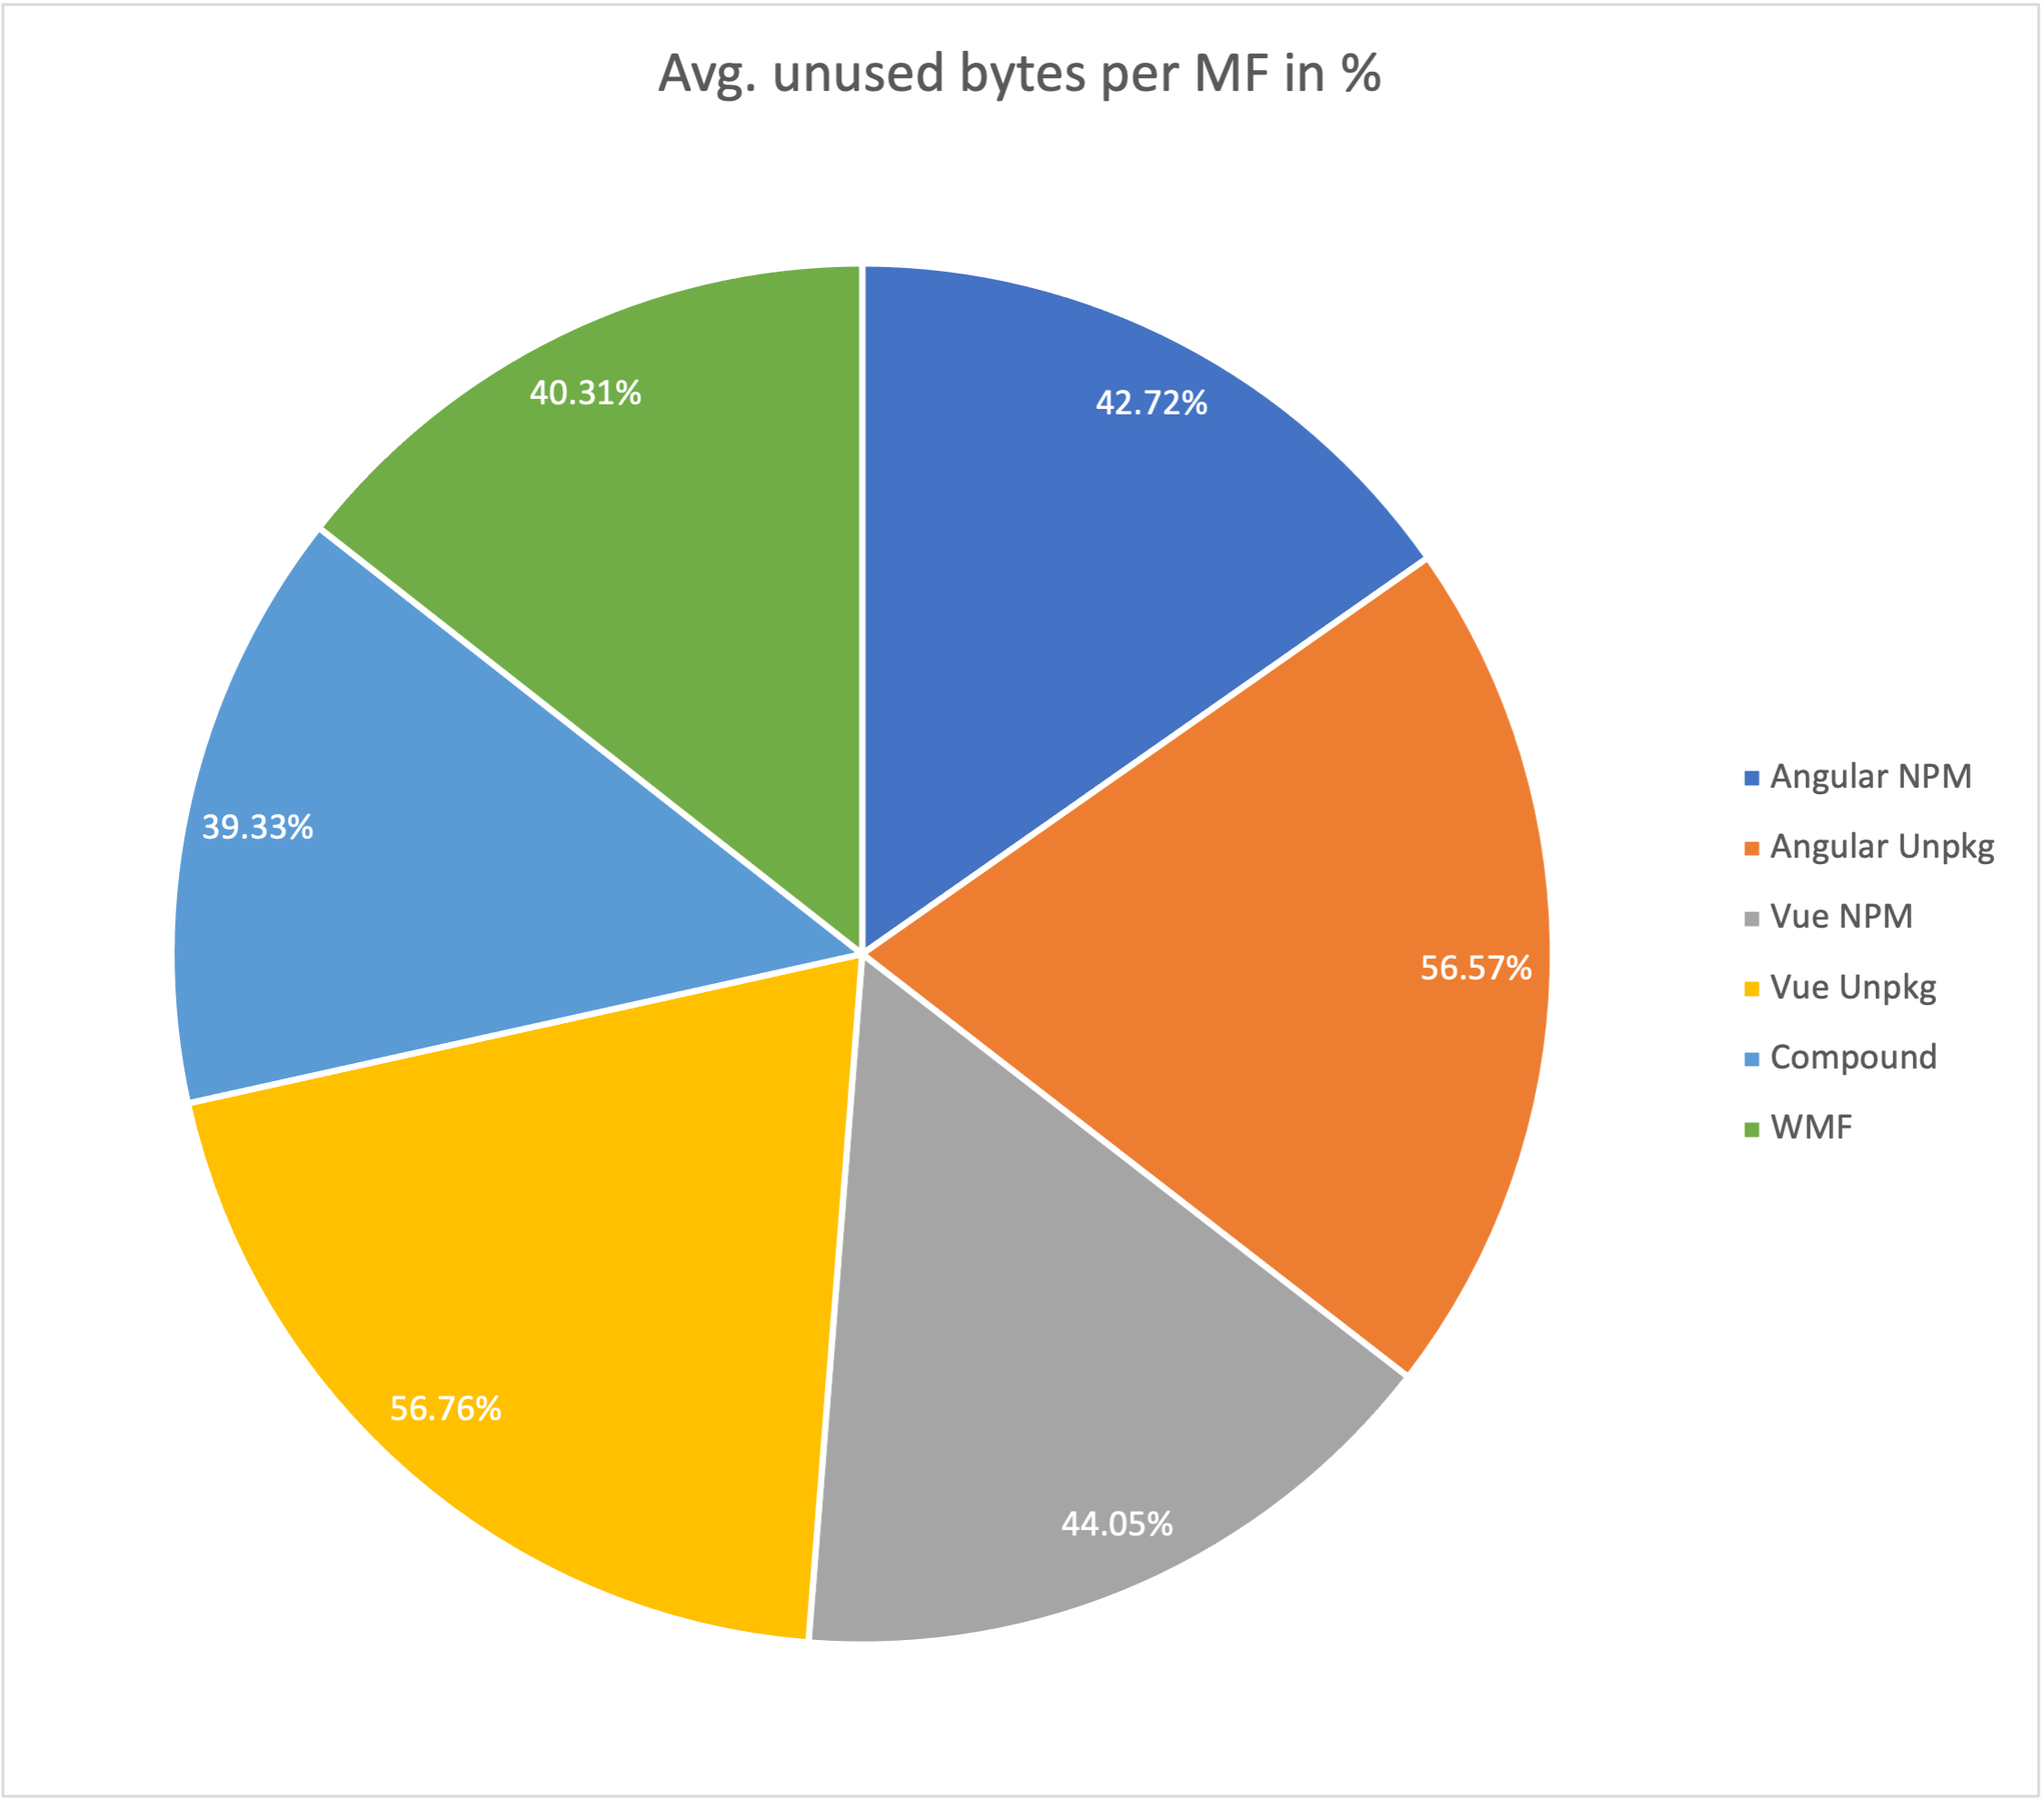
\includegraphics[width=1\textwidth]{Figures/avg_unsed_imported_2.png}
	\caption{Unused and imported bytes per landscape}
	\label{fig:unsed_imported_1}
\end{figure}

%\begin{figure}[!h]
%	\centering
%	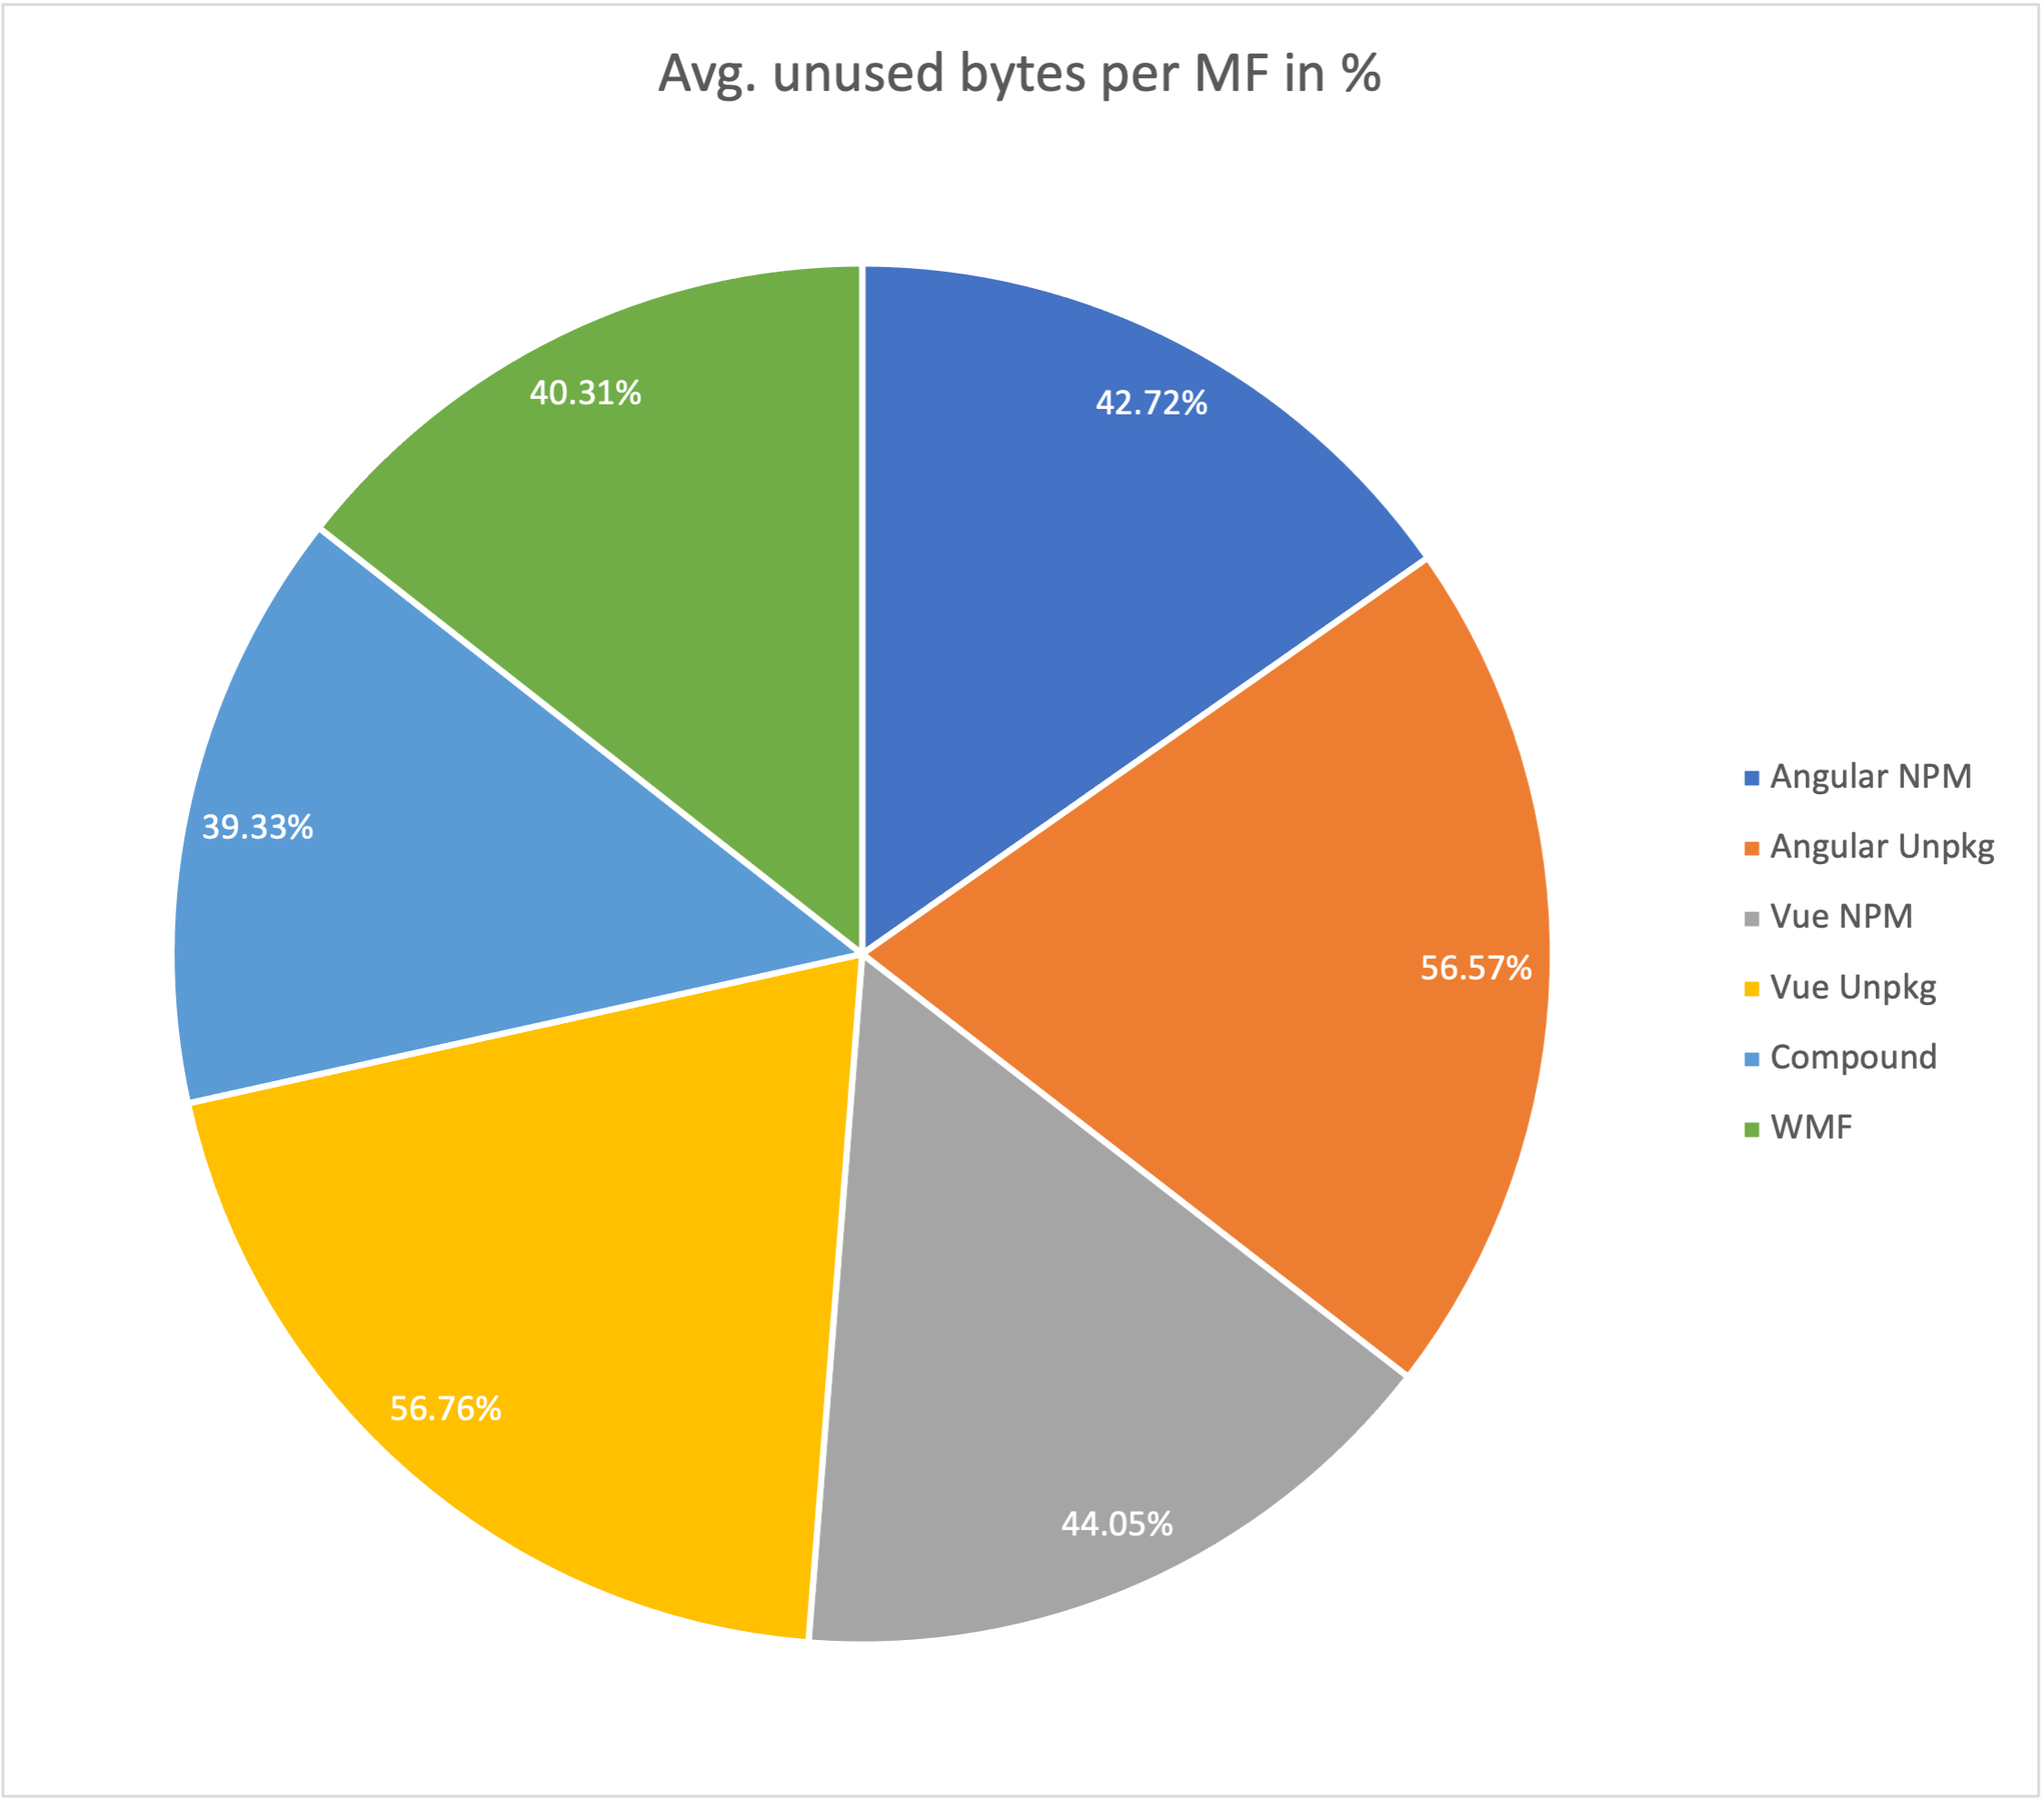
\includegraphics[width=1\textwidth]{Figures/avg_unsed_imported_2.png}
%	\caption{Unused and imported bytes per landscape in \%}
%	\label{fig:unsed_imported_2}
%\end{figure}

\normalsize
The data in table \ref{tab:lighthouse_used_report} and figure \ref{fig:unsed_imported_1} is highly application-dependent. 
As these landscapes are considered to be generally representative, a display in efficiency can be drawn from the charts.
The Unpkg CDN Nodes show a high ratio of unused bytes. 
However, it has to be taken into account that the overall imported sum of bytes is lower compared to the NPM counterparts, since only the required resources were requested from the CDN.
For the WMF Nodes, it can be argued that due to the bundling with Webpack, a lot of bytes were imported and only a few of them were not used. 
This can be explained by how the Module Federation was configured for this prototype. 
To simulate a multi-version landscape, a rather restrictive WMF configuration was required. 
Therefore, the majority of the bundled dependencies is actually used by the modules in those landscapes.
Web Components have the lowest unused bytes ratio of all the Nodes. 
This might be due to the fact that no UI framework was used for development. 
Therefore, no unnecessary framework features are present in this landscape.

The following chapter will draw conclusions based on the displayed data. Detailed tables, code examples and further information can be found in the archive.
